%
% File acl2020.tex
%
%% Based on the style files for ACL 2020, which were
%% Based on the style files for ACL 2018, NAACL 2018/19, which were
%% Based on the style files for ACL-2015, with some improvements
%%  taken from the NAACL-2016 style
%% Based on the style files for ACL-2014, which were, in turn,
%% based on ACL-2013, ACL-2012, ACL-2011, ACL-2010, ACL-IJCNLP-2009,
%% EACL-2009, IJCNLP-2008...
%% Based on the style files for EACL 2006 by 
%%e.agirre@ehu.es or Sergi.Balari@uab.es
%% and that of ACL 08 by Joakim Nivre and Noah Smith

\documentclass[11pt,a4paper]{article}
\usepackage[hyperref]{acl2020}
\usepackage{times}
\usepackage{latexsym}
\renewcommand{\UrlFont}{\ttfamily\small}

% This is not strictly necessary, and may be commented out,
% but it will improve the layout of the manuscript,
% and will typically save some space.
\usepackage{microtype}
\usepackage{graphicx}
\graphicspath{ {images/} }
\raggedbottom
\usepackage{colortbl}

\aclfinalcopy % Uncomment this line for the final submission
%\def\aclpaperid{***} %  Enter the acl Paper ID here

%\setlength\titlebox{5cm}
% You can expand the titlebox if you need extra space
% to show all the authors. Please do not make the titlebox
% smaller than 5cm (the original size); we will check this
% in the camera-ready version and ask you to change it back.

\newcommand\BibTeX{B\textsc{ib}\TeX}

\title{Evaluating the Efficacy of Attention Mechanisms on the Captioning of Images Taken by Visually Impaired People}

\author{Catherine Viloria \\
  University of Gothenburg \\ 
  \texttt{gusviloca@student.gu.se}}

\date{}

\begin{document}
\maketitle
\begin{abstract}
yaaa
\end{abstract}

\section{Introduction}

Image caption generation continues to be a pertinent task within both the computer vision community and the natural language processing (NLP) research field. However, it is important for researchers to also consider how advancements in this field can and will affect users in the real world. Developing models that will be able to effectively and efficiently assist visually impaired users in their day-to-day lives is a challenge in the field to this day. Models that are considered to have a high performance in automatically generating captions will not necessarily perform well in a domain-specific task. Captions for the visually impaired must be detailed yet concise and prioritise the objects of interest within the image. Another factor that could affect a model’s performance would be the quality of the images that are typically associated with caption generation for this task. It is not uncommon for images to be in the wrong orientation, unfocused, and out of frame. While any improvement in image captioning is still a step forward, critically examining applications of these models in situations that are not as contrived is extremely important. 

In this project, the VizWiz dataset presented by \citet{Gurari-2020-captioning}, specifically created to represent the blind and visually impaired community, is used to train an encoder-decoder model with attention to examine how a standard image captioning model will perform in generating captions for the visually impaired. Evaluating the neural image caption generator with visual attention presented by \citet{Xu-2015-show-attend} through a domain-specific lens is important for the community being affected but also will have research-related contributions. Choosing to assess a model in this way presents nuances that are sometimes overlooked when implementing these models. It will also shed light on how humans would approach a task and eventually the possibility of replicating said modus operandi or intuition in a model. The problem of the gap between the two modalities—image and text—presented in \citet{Bernardi-2016-automatic} is also discussed. The extent of how bad this problem will be in this model is shown to be exacerbated because of the dataset used since grounding becomes an even more difficult task. 

The following sections are organised as follows. Section 2 introduces image caption generation and the models and attention mechanism that precede what was implemented for this paper. In Section 3, the VizWiz dataset and specifics of the model implementation are given. The results are presented in Section 4. Section 5 discusses the results. Specific plans for future work are defined in Section 6 and it is followed by the conclusion and future work in Section 7. References are provided in Section 8.

\section{Related Work}
Automatic description generation from images has been a challenging task that both the computer vision and natural language processing communities have taken an interest in. \citet{Bernardi-2016-automatic} surveys the current approaches to this task and classifies these approaches through how they conceptualise the problem—either a generation problem, a retrieval from a visual space problem, or a retrieval from a multimodal space problem. All three approaches have their advantages and disadvantages. The first two approaches choose to rely more heavily on one modality (visual or textual) to base the predictions for generating captions while the third approach attempts to combine both representations to make the final image description. The implementation in this paper is the third approach. This approach attempts to address the semantic gap or mapping problem between language and image representations through the attentional component. The attention mechanism allows us to see visualizations of which regions in an image are salient and where the model is “looking” when generating each word in the caption.

The model implemented in this paper is a combination of proposed methods from two different, but related, research areas—image captioning and machine translation. \citet{Vinyals-2014-showandtell}’s seminal paper \emph{Show and Tell} presents a neural image caption generator (NIC) that uses a vision convolutional neural network (CNN) that encodes images with richer representations to a fixed dimension for the decoder. The encoder’s output is then passed to a language-generating recurrent neural network (RNN)—an LSTM-based sentence generator. Their model demonstrates that this approach significantly improves both accuracy and fluency when generating captions. A neural machine translation with an attention mechanism is proposed in \citet{Bahdanau-2014-neural}. Attention allows the model to look for parts in the source sentence that would be most relevant in predicting the target word. The flexibility of alignment between the source and target sentences introduced through attention allows for better translations, especially between languages that have syntactical differences. 

The combination of NIC and an attention mechanism resulted in the model implemented by \citet{Xu-2015-show-attend}—a neural image caption generator with visual attention. The encoder uses low-level representations which prioritises salient features of an image. The attention component adds “an extra layer of interpretability to the output of the model” \citep{Xu-2015-show-attend} and the alignments learned by the model correspond very well with human intuition. The motivations and intuitions of choosing to use the model implemented by \citet{Xu-2015-show-attend} for this domain-specific task is discussed in Section 3. 


\section{Dataset \& Methodology}
\subsection{VizWiz Dataset}
The domain-specific dataset used for this project was the VizWiz dataset \footnote{\url{https://vizwiz.org/}}. It is comprised of 39,181 images taken by people who are either blind or visually impaired. The images of the dataset come from a mobile phone application made to support real-world users through their visual description service. Users take a picture, record a spoken question and are then connected with people that could assist them. The VizWiz dataset has also been developed for various computer vision tasks, all related and extremely useful for the visually impaired community: image captioning, image quality assessment, visual question answering (VQA), answer-difference reasoning, vision skills for VQA, and visual privacy recognition. The VizWiz dataset is “a valuable foundation for designing more generalized computer vision algorithms that meet the large diversity of needs for real end users” \citep{Gurari-2020-captioning}. 

\subsubsection{VizWiz-Captions Dataset}
For this project, the VizWiz-Captions dataset \footnote{\url{https://vizwiz.org/tasks-and-datasets/image-captioning/}} was used. Each image is paired with 5 human-made captions collected through crowdsourcing via Amazon Mechanical Turk. Due to GPU limitations and consciousness of memory usage, only the training dataset was used. The training dataset originally had 23,141 images and 117,155 captions. After examining some of the metadata included in the dataset, a filtering process was conducted. If an image was considered to be spam (\emph{is\_rejected} column) or considered to have quality issues by annotators (\emph{is\_precanned} column, if True had “Quality issues are too severe to recognize visual content.” as its caption), they were filtered out of the dataset. Images with the characteristic of having text were kept since text is one of the main reasons why someone who is visually impaired would need assistance. After filtering, there were 14,790 images left and the model implementation was done with a 60/20/20 train, validation, test split (8,874 train, 2,958 validation, and 2,958 test).

\subsubsection{Annotator Reliability \& Ethical Considerations}
Although it is incredibly important to collect human-made captions for any text generation task, the process and its output also present some challenges and factors that must be considered. While it is greatly advantageous for a model to learn from human-made captions, humans are not perfect and also make mistakes. Crowdsourcing allows researchers to reach a larger, more widespread and diverse demographic but it also makes it much more difficult to oversee and guide annotators to ensure that the captions being made are of the best quality. The instructions provided to annotators presented in \citet{Gurari-2020-captioning}, while understandably so given the conditions of the annotation process, were very concise and left space for restrictions on the annotators that would affect the dataset and future model implementations.  

Examples of instructions that could lead to problems when training models are: “Include at least eight words.”, “Describe all parts of the image that may be important to a person who is blind.”, and “If text is in the image, and is important, then you can summarize what it says. DO NOT use all the specific phrases that you see in the image as your description of the image.” \citep{Gurari-2020-captioning} If an annotator was able to effectively describe an image with 4 words (e.g. “Can of mushroom soup.”), they are then required to add additional information that might not be neither useful nor necessary. The second instruction can also be interpreted as subjective and what one annotator thinks is useful information for a person who is blind, another annotator might not think similarly. Finally, the third instruction requiring a summarization of text that appears in an image rather than providing a word-for-word description makes it extremely difficult to ground any generated caption for a model. Although text summarization would be useful for this real-world task, it is a completely different task that is overlooked when training an image caption generator. 

Since annotators were also found through crowdsourcing, annotator reliability could possibly be a point of contention. Not only are the annotators’ backgrounds unknown, they are also inconsistent. In an ideal world, it would have been better to have real-world users with high ratings of the mobile application to come in and annotate images as they have domain-specific knowledge and skills. Ethical concerns may also affect the quality of work annotators submit. It is extremely important to acknowledge the absolutely dismal wages provided to annotators through Amazon Mechanical Turk.\citep{hara2018amazon} The low wages and absence of work benefits can also affect the care and quality of the captions made by annotators. With these considerations, an example is provided in \autoref{fig:vwcaption} of how varied and inconsistent the quality and structure of captions can be within the dataset. The variation in complexity and length is quite large and can be argued to be either advantageous or disadvantageous for a model when training. 

\begin{figure}[h]
  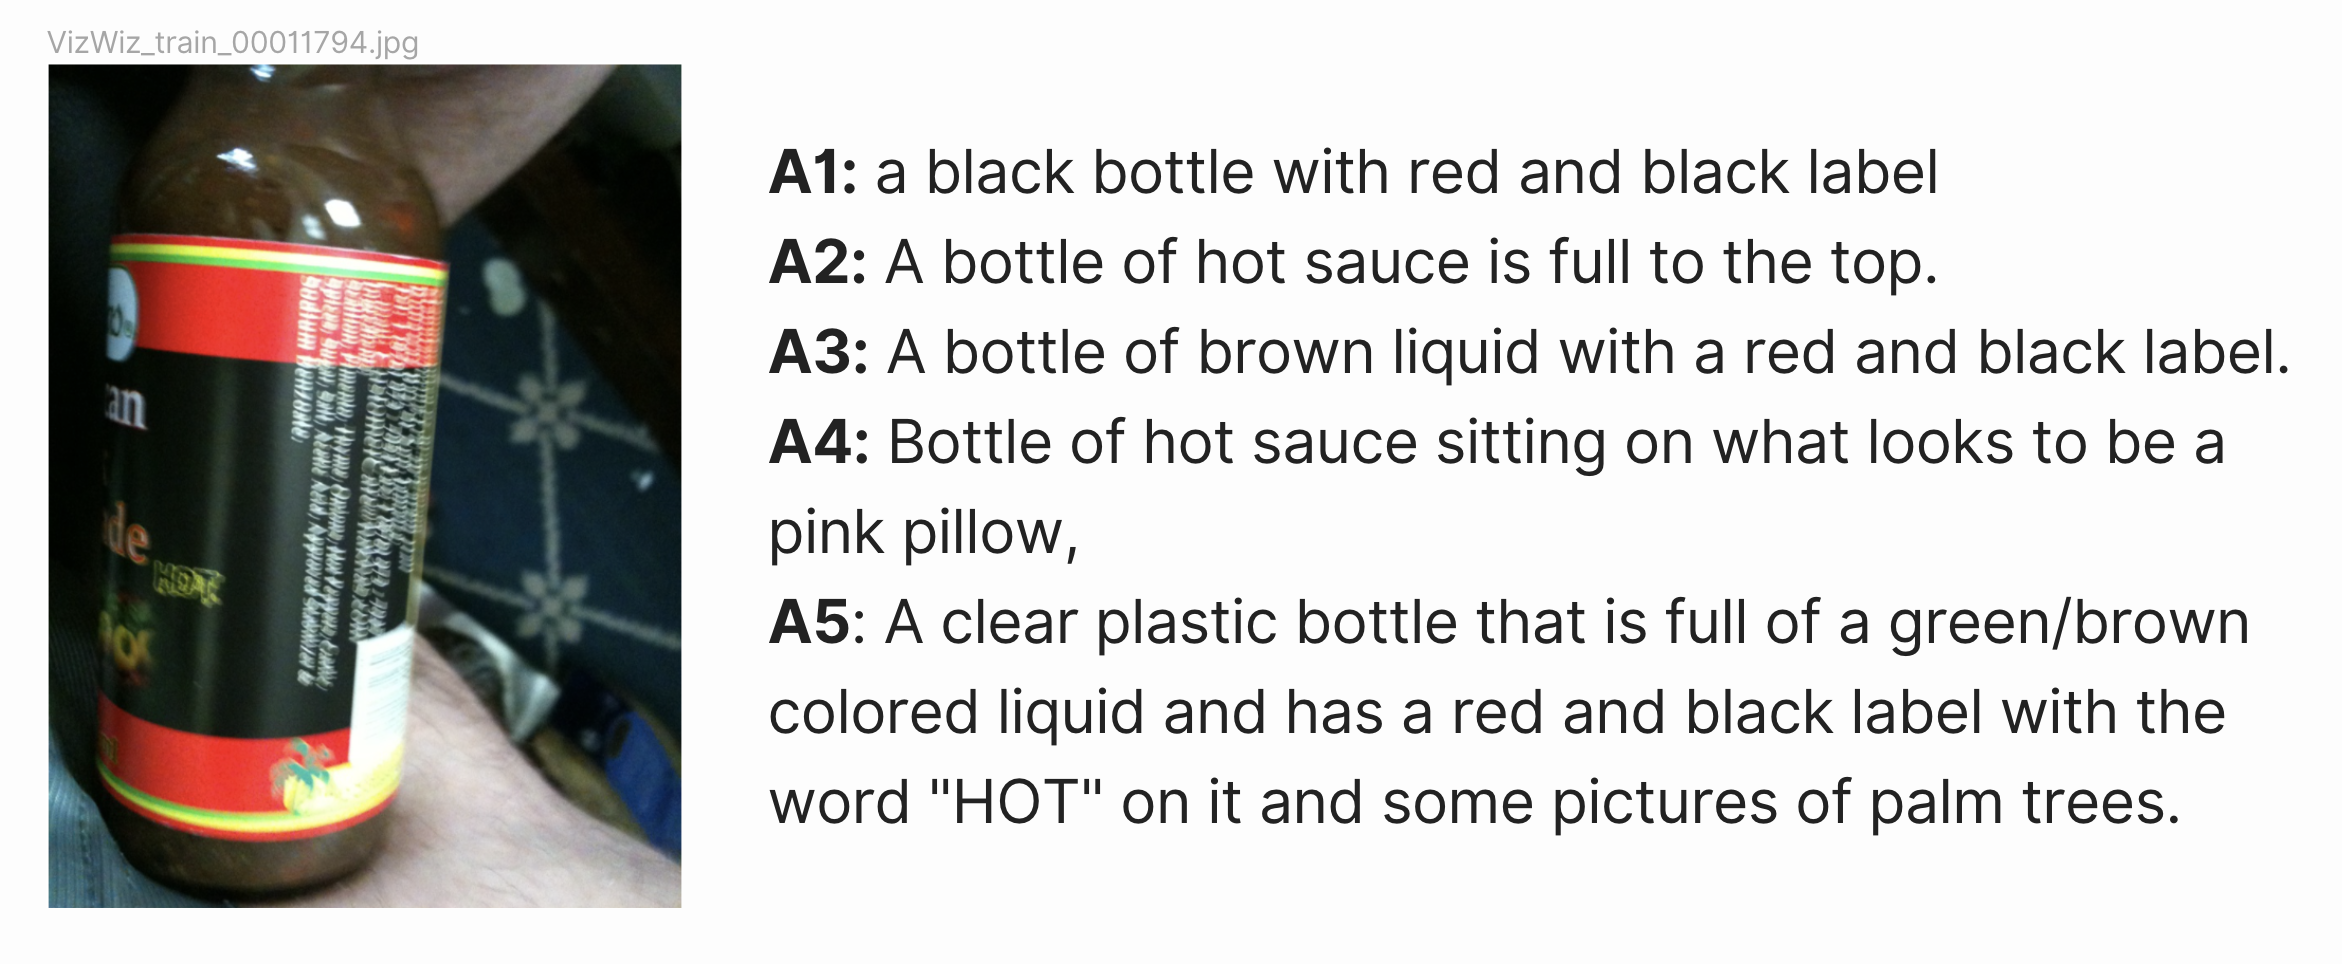
\includegraphics[width=\linewidth]{VizWiz_train_00011794_captioned.png}
  \caption{An image from the VizWiz-Captions dataset and 5 captions from 5 different annotators.}
  \label{fig:vwcaption}
\end{figure}

\subsection{Model Architecture}
The model implemented was an encoder-decoder with an attention mechanism. The PyTorch Tutorial to Image Captioning by Sagar Vinodababu\footnote{\url{https://github.com/sgrvinod/a-PyTorch-Tutorial-to-Image-Captioning#training}} was followed and the implementation included an encoder that was pretrained on ResNet. The encoder is responsible for taking the images as input and transforming it into smaller representations. It returns a “state” that is fed into the decoder. The decoder is then responsible for interpreting the output of the encoder. It also calculates the attention weights for the image. (*also generates caption/ language model??)

Creating low-level representations when passed through the encoder seemed like a good approach for this task since a lot of images in the dataset only have one object as the focal point and this object is only partially shown in the image. A lower-level representation or a representation that is closer to what the image actually looks like would be very helpful rather than having a representation that is an average of everything in the picture. This approach would be called the top-down approach—contrasted with the bottom-up approach which is good for semantically-rich images where multiple objects within the image are first identified and then given to the encoder. Datasets that have high-quality and semantically-rich images, such as MSCOCO, are more ideal for the top-down approach.**NEED TO REFER TO ANDERSON (2018)??? 

During training, sequences are padded then ordered by length in order to minimise computations (****???wording). Word embeddings, attention weights, and the decoder all have a dimension of 512 with a batch size of 32. The encoder’s learning rate was 0.0001 and the decoder’s learning rate was 0.0004. Early stopping was implemented after 20 epochs of no improvement. These hyperparameters and implementations were all chosen through the tutorial source.  

The greedy search algorithm was implemented for generating captions. In the greedy search algorithm, when given a number of choices in the next stage, the model will always choose the best immediate output. For this task, the language model takes the vocabulary’s logits and turns them into probabilities. This is then fed to the greedy search algorithm where it chooses the highest probable word to occur next at each stage. However, greedy search also has its drawbacks. Since it only chooses the best immediate output and does not look farther ahead, it has a higher chance of not reaching the globally optimum solution—hence its name, \emph{greedy} search.

\section{Results}
\label{sec:results}
ya ya look at  \autoref{trainingdata} that shows

% training stats table
\begin{table}
\centering
\begin{tabular}{|c|c|c|} 
\hline
\rowcolor[rgb]{0.761,0.761,0.761} \textbf{Epochs} & \textbf{Top-5 Accuracy} & \textbf{BLEU-4}  \\ 
\hline
0                                                 & 55.982                  & 0.1047           \\ 
\hline
1                                                 & 59.216                  & 0.1180           \\ 
\hline
2                                                 & 60.894                  & 0.1277           \\ 
\hline
3                                                 & 62.122                  & 0.1307           \\ 
\hline
4                                                 & 62.798                  & 0.1362           \\ 
\hline
5                                                 & 63.192                  & 0.1371           \\ 
\hline
6                                                 & 63.632                  & 0.1404           \\ 
\hline
7                                                 & 63.87                   & 0.1429           \\ 
\hline
8                                                 & 64.06                   & 0.1421           \\ 
\hline
9                                                 & 64.045                  & 0.1440           \\ 
\hline
10                                                & 64.1                    & 0.1447           \\ 
\hline
11                                                & 64.112                  & 0.1449           \\ 
\hline
12                                                & 64.193                  & 0.1451           \\ 
\hline
13                                                & 64.031                  & 0.1445           \\ 
\hline
\rowcolor[rgb]{0.992,0.992,0.588} 14              & 63.923                  & 0.1465           \\ 
\hline
15                                                & 63.912                  & 0.1461           \\ 
\hline
16                                                & 63.808                  & 0.1460           \\ 
\hline
17                                                & 63.753                  & 0.1459           \\ 
\hline
18                                                & 63.526                  & 0.1456           \\ 
\hline
19                                                & 63.594                  & 0.1452           \\ 
\hline
20                                                & 63.283                  & 0.1427           \\ 
\hline
21                                                & 63.275                  & 0.1429           \\ 
\hline
22                                                & 62.96                   & 0.1434           \\ 
\hline
23                                                & 63.015                  & 0.1421           \\ 
\hline
24                                                & 62.811                  & 0.1422           \\ 
\hline
25                                                & 62.629                  & 0.1419           \\ 
\hline
26                                                & 62.436                  & 0.1423           \\ 
\hline
27                                                & 62.424                  & 0.1416           \\ 
\hline
28                                                & 62.383                  & 0.1400           \\ 
\hline
29                                                & 62.144                  & 0.1383           \\ 
\hline
30                                                & 62.031                  & 0.1403           \\ 
\hline
31                                                & 62.002                  & 0.1382           \\ 
\hline
32                                                & 61.882                  & 0.1389           \\ 
\hline
33                                                & 61.649                  & 0.1370           \\ 
\hline
34                                                & 61.53                   & 0.1383           \\
\hline
\end{tabular}
\caption{\label{trainingdata}Top-5 accuracy and BLEU-4 score after each epoch during training. The row highlighted in yellow is the model that performed the best and what was used for validation and testing.}
\end{table}
% ------end of table------

and see the loss curve in \autoref{fig:lossgraph}


% loss graph figure
\begin{figure}[h]
  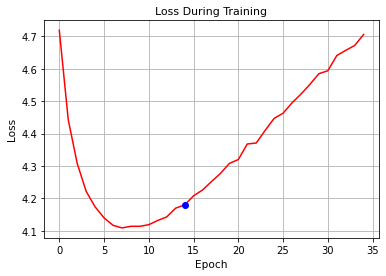
\includegraphics[width=\linewidth]{paper/images/loss_graph.png}
  \caption{Loss curve during training. The blue point is the loss for the best performing model.}
  \label{fig:lossgraph}
\end{figure}
% ----end of figure----


% examples of captions
\begin{quote}
  ``white background''
\end{quote}
\begin{quote}
  ``a close up of a white background with a black background''
\end{quote}
\begin{quote}
  ``a close up of a black background with a white background with a white background''
\end{quote}
\begin{quote}
  ``a close up of a black background with black lettering''
\end{quote}
\begin{quote}
  ``the photo is cropped out of the frame''
\end{quote}

% attention - black screen
\begin{figure}[h]
  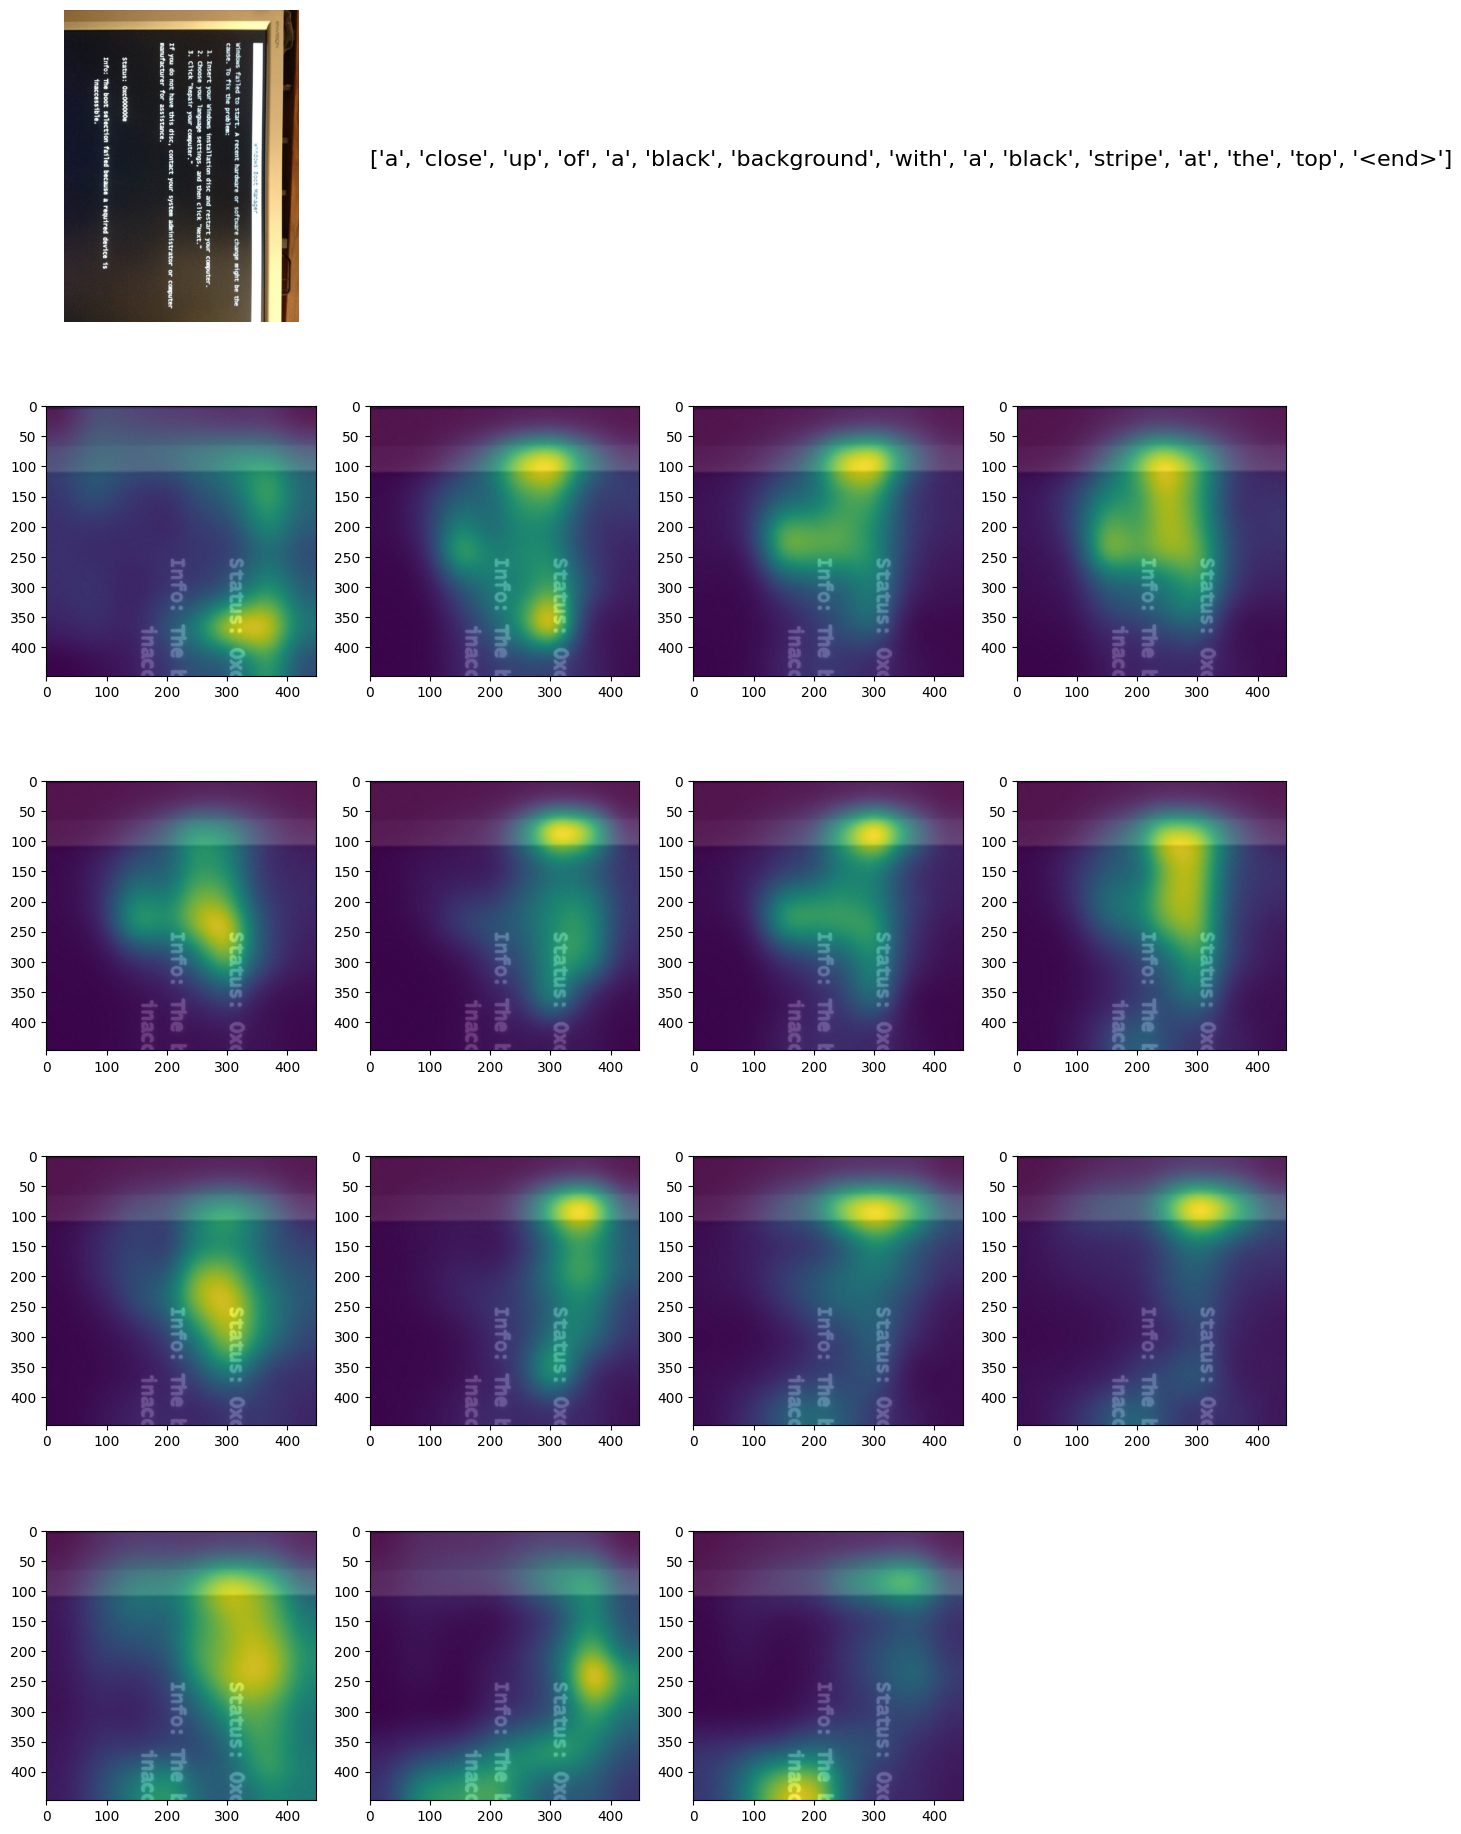
\includegraphics[width=\linewidth]{VizWiz_train_00000858.png}
  \caption{black screen}
  \label{fig:blackscreen}
\end{figure}
% ----end of figure----

% attention - stapler
\begin{figure}[h]
  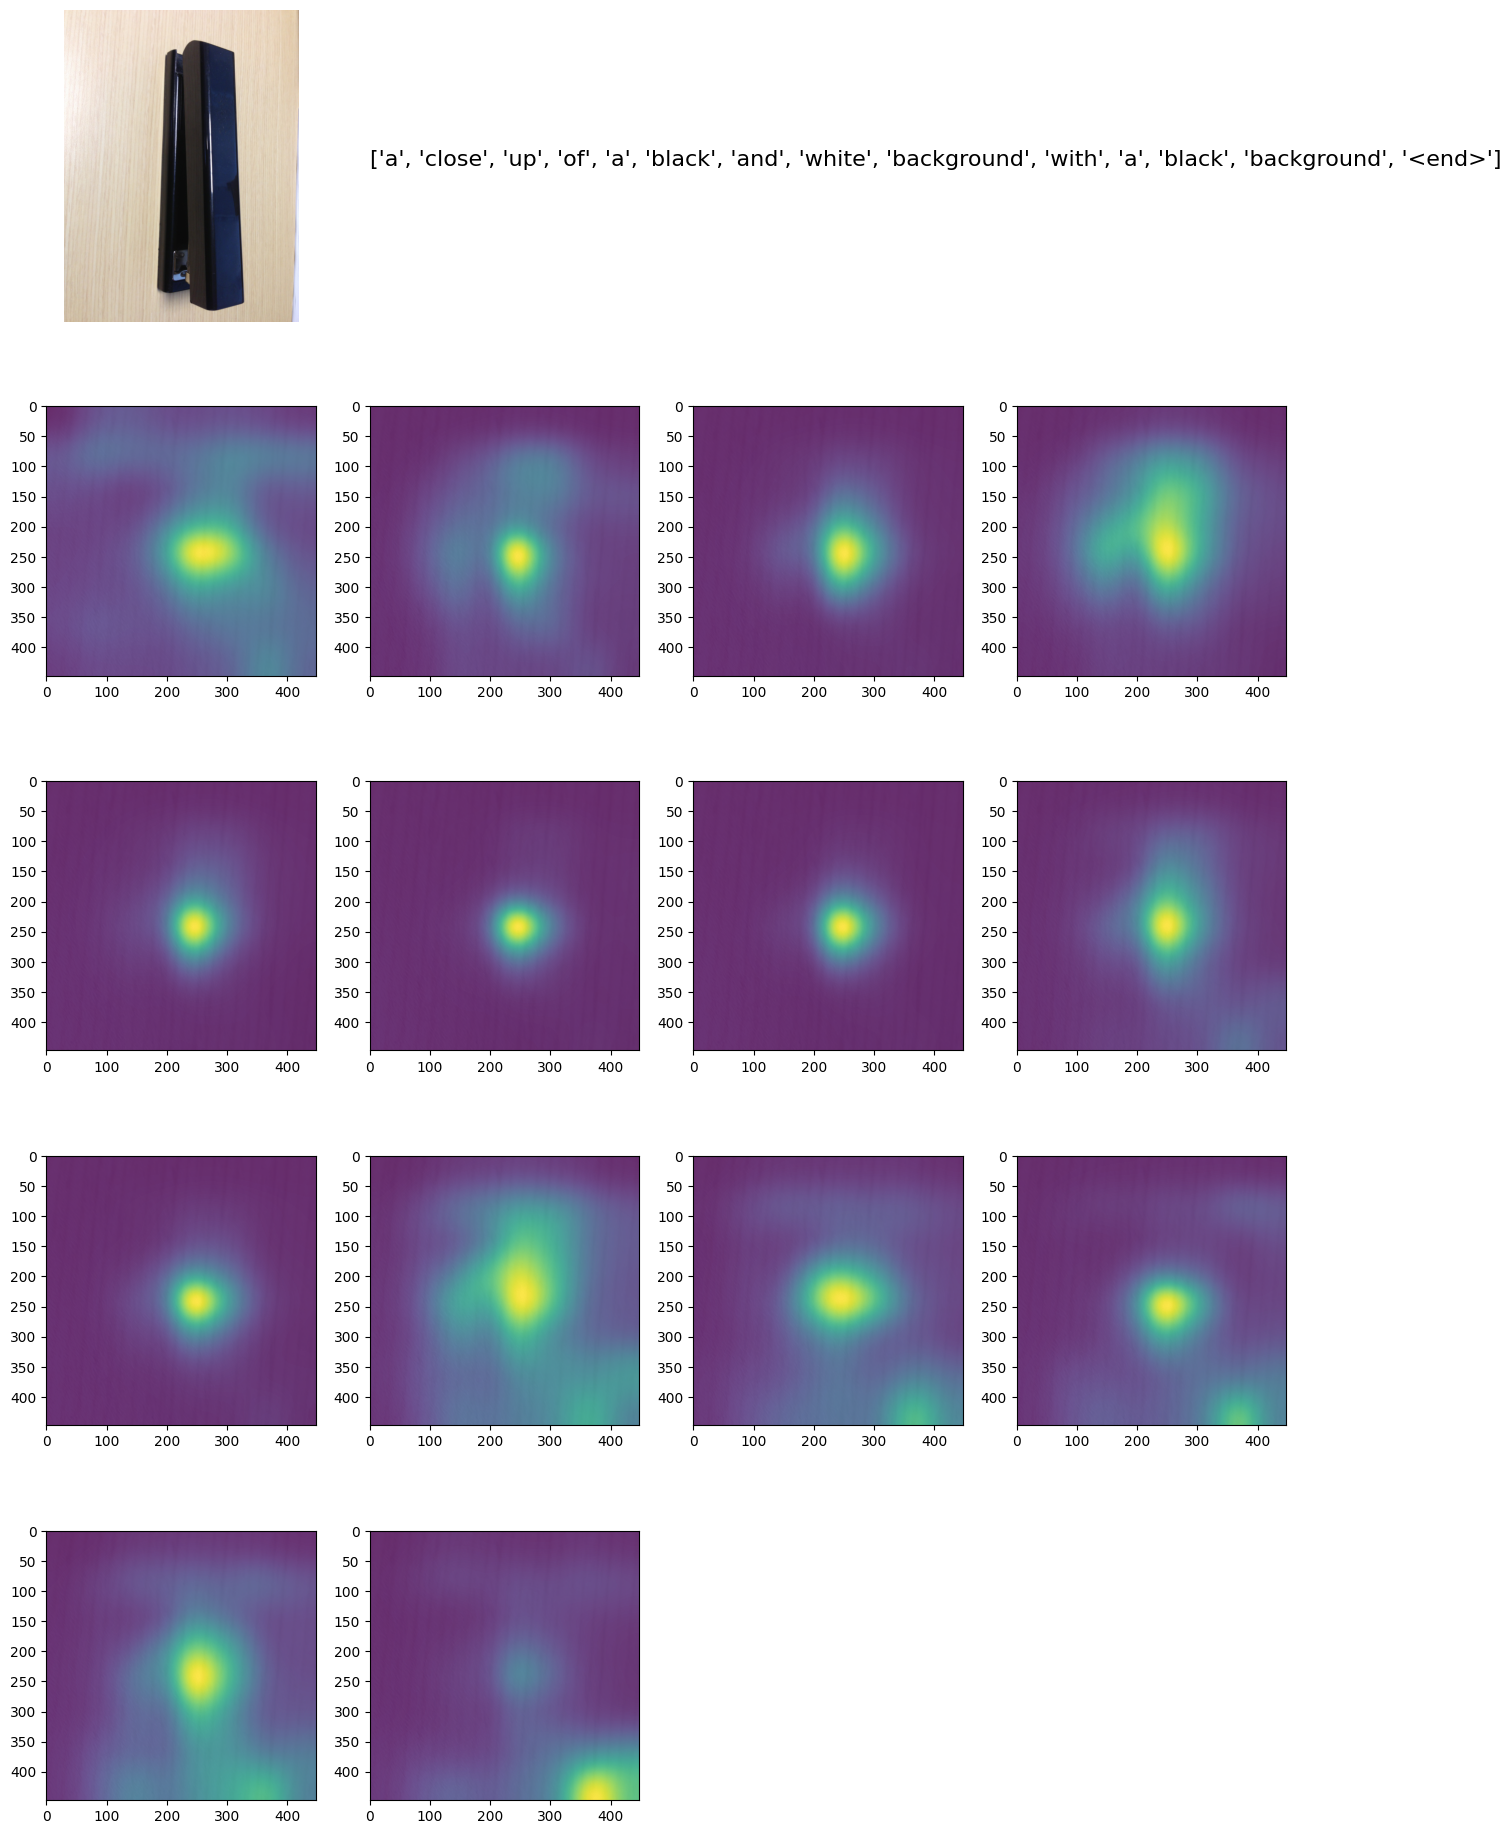
\includegraphics[width=\linewidth]{VizWiz_train_00013366.png}
  \caption{example}
  \label{fig:stapler}
\end{figure}
% ----end of figure----

% attention - whitetext
\begin{figure}[h]
  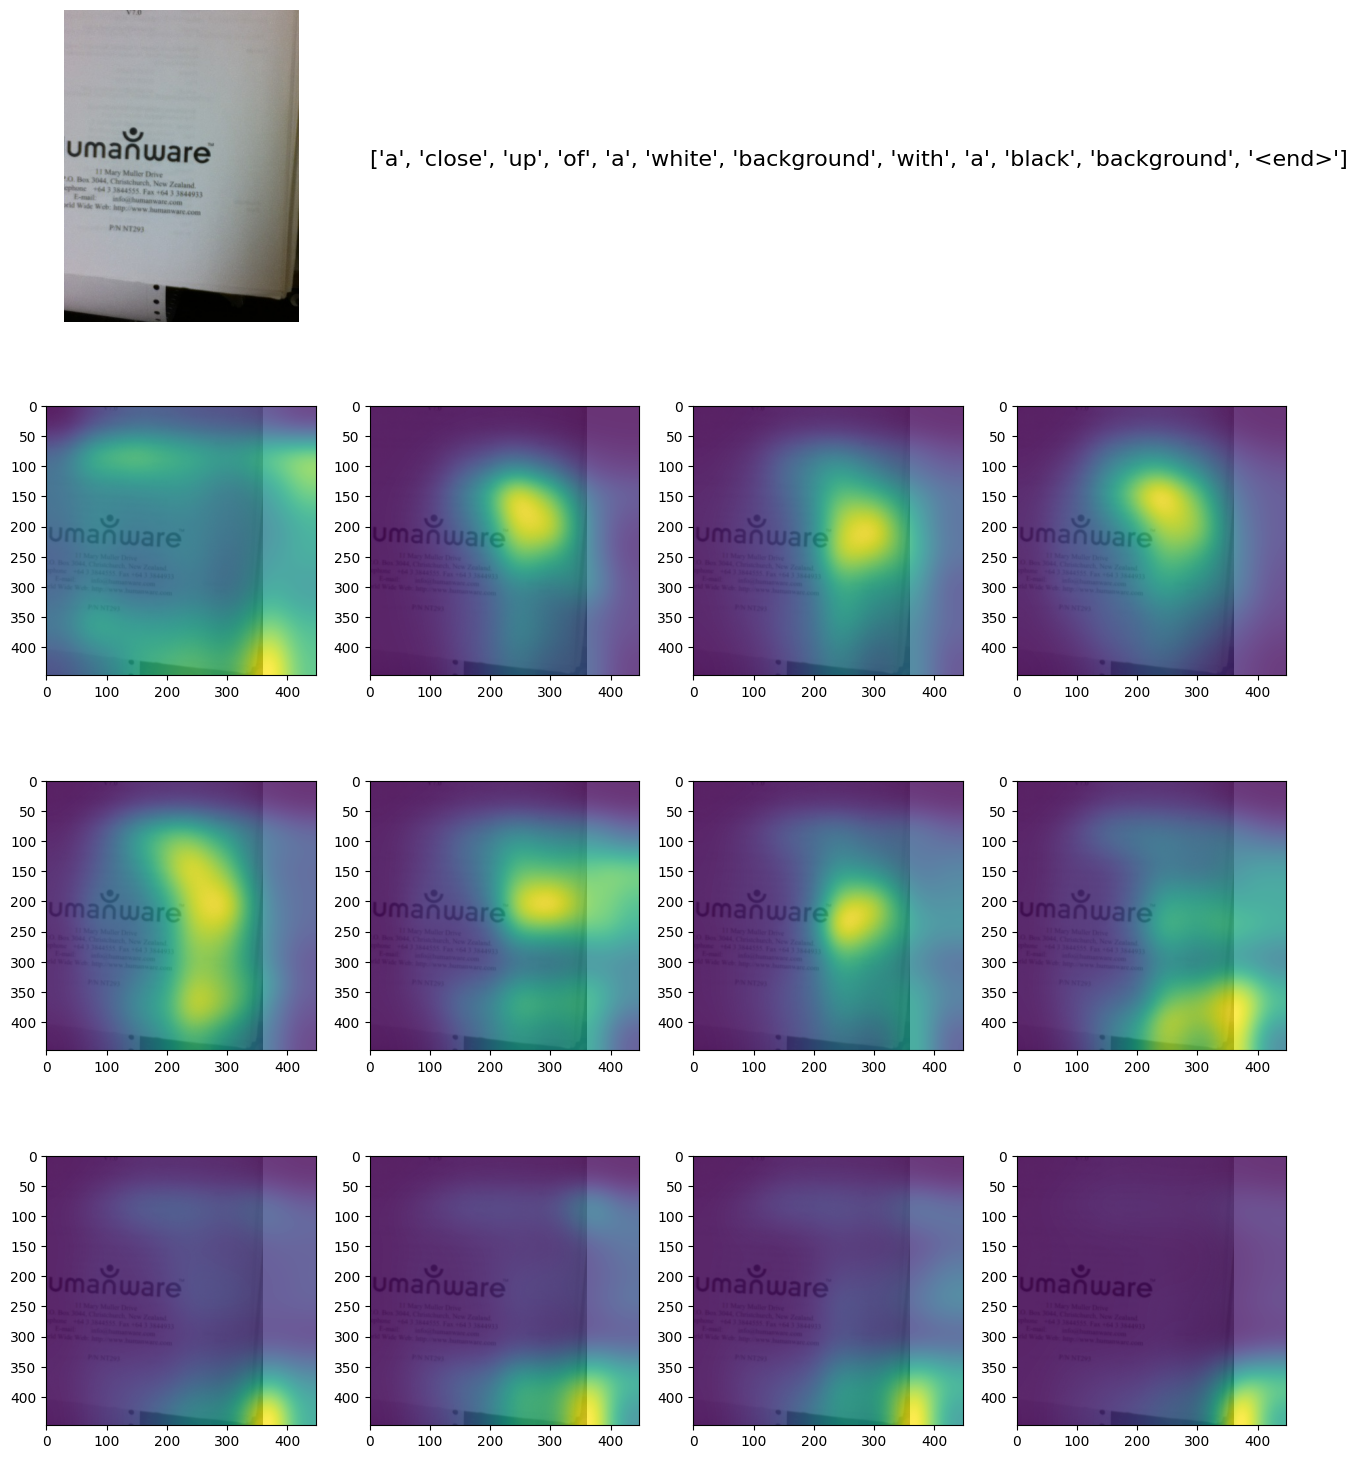
\includegraphics[width=\linewidth]{VizWiz_train_00023423.png}
  \caption{page with text}
  \label{fig:whitetext}
\end{figure}
% ----end of figure----

\section{Discussion}
As reviewing will be double-blind, papers submitted for review should not include any author information (such as names or affiliations). Furthermore, self-references that reveal the author's identity, \emph{e.g.},
\begin{quote}
We previously showed \citep{Gusfield:97} \ldots
\end{quote}
should be avoided. Instead, use citations such as 
\begin{quote}
\citet{Gusfield:97} previously showed\ldots
\end{quote}
Please do not use anonymous citations and do not include acknowledgements.
\textbf{Papers that do not conform to these requirements may be rejected without review.}

Any preliminary non-archival versions of submitted papers should be listed in the submission form but not in the review version of the paper.
Reviewers are generally aware that authors may present preliminary versions of their work in other venues, but will not be provided the list of previous presentations from the submission form.

Once a paper has been accepted to the conference, the camera-ready version of the paper should include the author's names and affiliations, and is allowed to use self-references.

\paragraph{\LaTeX-specific details:}
For an anonymized submission, ensure that {\small\verb|\aclfinalcopy|} at the top of this document is commented out, and that you have filled in the paper ID number (assigned during the submission process on softconf) where {\small\verb|***|} appears in the {\small\verb|\def\aclpaperid{***}|} definition at the top of this document.
For a camera-ready submission, ensure that {\small\verb|\aclfinalcopy|} at the top of this document is not commented out.


\section{Future Work}


\section{Conclusion}

Manuscripts must be in two-column format.
Exceptions to the two-column format include the title, authors' names and complete addresses, which must be centered at the top of the first page, and any full-width figures or tables (see the guidelines in Section~\ref{ssec:title-authors}).
\textbf{Type single-spaced.}
Start all pages directly under the top margin.
The manuscript should be printed single-sided and its length should not exceed the maximum page limit described in Section~\ref{sec:length}.
Pages should be numbered in the version submitted for review, but \textbf{pages should not be numbered in the camera-ready version}.

\paragraph{\LaTeX-specific details:}
The style files will generate page numbers when {\small\verb|\aclfinalcopy|} is commented out, and remove them otherwise.


\subsection{File Format}
\label{sect:pdf}

For the production of the electronic manuscript you must use Adobe's Portable Document Format (PDF).
Please make sure that your PDF file includes all the necessary fonts (especially tree diagrams, symbols, and fonts with Asian characters).
When you print or create the PDF file, there is usually an option in your printer setup to include none, all or just non-standard fonts.
Please make sure that you select the option of including ALL the fonts.
\textbf{Before sending it, test your PDF by printing it from a computer different from the one where it was created.}
Moreover, some word processors may generate very large PDF files, where each page is rendered as an image.
Such images may reproduce poorly.
In this case, try alternative ways to obtain the PDF.
One way on some systems is to install a driver for a postscript printer, send your document to the printer specifying ``Output to a file'', then convert the file to PDF.

It is of utmost importance to specify the \textbf{A4 format} (21 cm x 29.7 cm) when formatting the paper.
Print-outs of the PDF file on A4 paper should be identical to the hardcopy version.
If you cannot meet the above requirements about the production of your electronic submission, please contact the publication chairs as soon as possible.

\paragraph{\LaTeX-specific details:}
PDF files are usually produced from \LaTeX{} using the \texttt{\small pdflatex} command.
If your version of \LaTeX{} produces Postscript files, \texttt{\small ps2pdf} or \texttt{\small dvipdf} can convert these to PDF.
To ensure A4 format in \LaTeX, use the command {\small\verb|\special{papersize=210mm,297mm}|}
in the \LaTeX{} preamble (below the {\small\verb|\usepackage|} commands) and use \texttt{\small dvipdf} and/or \texttt{\small pdflatex}; or specify \texttt{\small -t a4} when working with \texttt{\small dvips}.

\subsection{Layout}
\label{ssec:layout}

Format manuscripts two columns to a page, in the manner these
instructions are formatted.
The exact dimensions for a page on A4 paper are:

\begin{itemize}
\item Left and right margins: 2.5 cm
\item Top margin: 2.5 cm
\item Bottom margin: 2.5 cm
\item Column width: 7.7 cm
\item Column height: 24.7 cm
\item Gap between columns: 0.6 cm
\end{itemize}

\noindent Papers should not be submitted on any other paper size.
If you cannot meet the above requirements about the production of your electronic submission, please contact the publication chairs above as soon as possible.

\subsection{Fonts}

For reasons of uniformity, Adobe's \textbf{Times Roman} font should be used.
If Times Roman is unavailable, you may use Times New Roman or \textbf{Computer Modern Roman}.

Table~\ref{font-table} specifies what font sizes and styles must be used for each type of text in the manuscript.

\begin{table}
\centering
\begin{tabular}{lrl}
\hline \textbf{Type of Text} & \textbf{Font Size} & \textbf{Style} \\ \hline
paper title & 15 pt & bold \\
author names & 12 pt & bold \\
author affiliation & 12 pt & \\
the word ``Abstract'' & 12 pt & bold \\
section titles & 12 pt & bold \\
subsection titles & 11 pt & bold \\
document text & 11 pt  &\\
captions & 10 pt & \\
abstract text & 10 pt & \\
bibliography & 10 pt & \\
footnotes & 9 pt & \\
\hline
\end{tabular}
\caption{\label{font-table} Font guide. }
\end{table}

\paragraph{\LaTeX-specific details:}
To use Times Roman in \LaTeX2e{}, put the following in the preamble:
\begin{quote}
\small
\begin{verbatim}
\usepackage{times}
\usepackage{latexsym}
\end{verbatim}
\end{quote}


\subsection{Ruler}
A printed ruler (line numbers in the left and right margins of the article) should be presented in the version submitted for review, so that reviewers may comment on particular lines in the paper without circumlocution.
The presence or absence of the ruler should not change the appearance of any other content on the page.
The camera ready copy should not contain a ruler.

\paragraph{Reviewers:}
note that the ruler measurements may not align well with lines in the paper -- this turns out to be very difficult to do well when the paper contains many figures and equations, and, when done, looks ugly.
In most cases one would expect that the approximate location will be adequate, although you can also use fractional references (\emph{e.g.}, this line ends at mark $295.5$).

\paragraph{\LaTeX-specific details:}
The style files will generate the ruler when {\small\verb|\aclfinalcopy|} is commented out, and remove it otherwise.

\subsection{Title and Authors}
\label{ssec:title-authors}

Center the title, author's name(s) and affiliation(s) across both columns.
Do not use footnotes for affiliations.
Place the title centered at the top of the first page, in a 15-point bold font.
Long titles should be typed on two lines without a blank line intervening.
Put the title 2.5 cm from the top of the page, followed by a blank line, then the author's names(s), and the affiliation on the following line.
Do not use only initials for given names (middle initials are allowed).
Do not format surnames in all capitals (\emph{e.g.}, use ``Mitchell'' not ``MITCHELL'').
Do not format title and section headings in all capitals except for proper names (such as ``BLEU'') that are
conventionally in all capitals.
The affiliation should contain the author's complete address, and if possible, an electronic mail address.

The title, author names and addresses should be completely identical to those entered to the electronical paper submission website in order to maintain the consistency of author information among all publications of the conference.
If they are different, the publication chairs may resolve the difference without consulting with you; so it is in your own interest to double-check that the information is consistent.

Start the body of the first page 7.5 cm from the top of the page.
\textbf{Even in the anonymous version of the paper, you should maintain space for names and addresses so that they will fit in the final (accepted) version.}


\subsection{Abstract}
Use two-column format when you begin the abstract.
Type the abstract at the beginning of the first column.
The width of the abstract text should be smaller than the
width of the columns for the text in the body of the paper by 0.6 cm on each side.
Center the word \textbf{Abstract} in a 12 point bold font above the body of the abstract.
The abstract should be a concise summary of the general thesis and conclusions of the paper.
It should be no longer than 200 words.
The abstract text should be in 10 point font.

\subsection{Text}
Begin typing the main body of the text immediately after the abstract, observing the two-column format as shown in the present document.

Indent 0.4 cm when starting a new paragraph.

\subsection{Sections}

Format section and subsection headings in the style shown on the present document.
Use numbered sections (Arabic numerals) to facilitate cross references.
Number subsections with the section number and the subsection number separated by a dot, in Arabic numerals.

\subsection{Footnotes}
Put footnotes at the bottom of the page and use 9 point font.
They may be numbered or referred to by asterisks or other symbols.\footnote{This is how a footnote should appear.}
Footnotes should be separated from the text by a line.\footnote{Note the line separating the footnotes from the text.}

\subsection{Graphics}

Place figures, tables, and photographs in the paper near where they are first discussed, rather than at the end, if possible.
Wide illustrations may run across both columns.
Color is allowed, but adhere to Section~\ref{ssec:accessibility}'s guidelines on accessibility.

\paragraph{Captions:}
Provide a caption for every illustration; number each one sequentially in the form:
``Figure 1. Caption of the Figure.''
``Table 1. Caption of the Table.''
Type the captions of the figures and tables below the body, using 10 point text.
Captions should be placed below illustrations.
Captions that are one line are centered (see Table~\ref{font-table}).
Captions longer than one line are left-aligned (see Table~\ref{tab:accents}).

\begin{table}
\centering
\begin{tabular}{lc}
\hline
\textbf{Command} & \textbf{Output}\\
\hline
\verb|{\"a}| & {\"a} \\
\verb|{\^e}| & {\^e} \\
\verb|{\`i}| & {\`i} \\ 
\verb|{\.I}| & {\.I} \\ 
\verb|{\o}| & {\o} \\
\verb|{\'u}| & {\'u}  \\ 
\verb|{\aa}| & {\aa}  \\\hline
\end{tabular}
\begin{tabular}{lc}
\hline
\textbf{Command} & \textbf{Output}\\
\hline
\verb|{\c c}| & {\c c} \\ 
\verb|{\u g}| & {\u g} \\ 
\verb|{\l}| & {\l} \\ 
\verb|{\~n}| & {\~n} \\ 
\verb|{\H o}| & {\H o} \\ 
\verb|{\v r}| & {\v r} \\ 
\verb|{\ss}| & {\ss} \\
\hline
\end{tabular}
\caption{Example commands for accented characters, to be used in, \emph{e.g.}, \BibTeX\ names.}\label{tab:accents}
\end{table}

\paragraph{\LaTeX-specific details:}
The style files are compatible with the caption and subcaption packages; do not add optional arguments.
\textbf{Do not override the default caption sizes.}


\subsection{Hyperlinks}
Within-document and external hyperlinks are indicated with Dark Blue text, Color Hex \#000099.

\subsection{Citations}
Citations within the text appear in parentheses as~\citep{Gusfield:97} or, if the author's name appears in the text itself, as \citet{Gusfield:97}.
Append lowercase letters to the year in cases of ambiguities.  
Treat double authors as in~\citep{Aho:72}, but write as in~\citep{Chandra:81} when more than two authors are involved. Collapse multiple citations as in~\citep{Gusfield:97,Aho:72}. 

Refrain from using full citations as sentence constituents.
Instead of
\begin{quote}
  ``\citep{Gusfield:97} showed that ...''
\end{quote}
write
\begin{quote}
``\citet{Gusfield:97} showed that ...''
\end{quote}

\begin{table*}
\centering
\begin{tabular}{lll}
\hline
\textbf{Output} & \textbf{natbib command} & \textbf{Old ACL-style command}\\
\hline
\citep{Gusfield:97} & \small\verb|\citep| & \small\verb|\cite| \\
\citealp{Gusfield:97} & \small\verb|\citealp| & no equivalent \\
\citet{Gusfield:97} & \small\verb|\citet| & \small\verb|\newcite| \\
\citeyearpar{Gusfield:97} & \small\verb|\citeyearpar| & \small\verb|\shortcite| \\
\hline
\end{tabular}
\caption{\label{citation-guide}
Citation commands supported by the style file.
The style is based on the natbib package and supports all natbib citation commands.
It also supports commands defined in previous ACL style files for compatibility.
}
\end{table*}

\paragraph{\LaTeX-specific details:}
Table~\ref{citation-guide} shows the syntax supported by the style files.
We encourage you to use the natbib styles.
You can use the command {\small\verb|\citet|} (cite in text) to get ``author (year)'' citations as in \citet{Gusfield:97}.
You can use the command {\small\verb|\citep|} (cite in parentheses) to get ``(author, year)'' citations as in \citep{Gusfield:97}.
You can use the command {\small\verb|\citealp|} (alternative cite without  parentheses) to get ``author year'' citations (which is useful for  using citations within parentheses, as in \citealp{Gusfield:97}).


\subsection{References}
Gather the full set of references together under the heading \textbf{References}; place the section before any Appendices. 
Arrange the references alphabetically by first author, rather than by order of occurrence in the text.

Provide as complete a citation as possible, using a consistent format, such as the one for \emph{Computational Linguistics\/} or the one in the  \emph{Publication Manual of the American 
Psychological Association\/}~\citep{APA:83}.
Use full names for authors, not just initials.

Submissions should accurately reference prior and related work, including code and data.
If a piece of prior work appeared in multiple venues, the version that appeared in a refereed, archival venue should be referenced.
If multiple versions of a piece of prior work exist, the one used by the authors should be referenced.
Authors should not rely on automated citation indices to provide accurate references for prior and related work.

The following text cites various types of articles so that the references section of the present document will include them.
\begin{itemize}
\item Example article in journal: \citep{Ando2005}.
\item Example article in proceedings, with location: \citep{borschinger-johnson-2011-particle}.
\item Example article in proceedings, without location: \citep{andrew2007scalable}.
\item Example arxiv paper: \citep{rasooli-tetrault-2015}. 
\end{itemize}


\paragraph{\LaTeX-specific details:}
The \LaTeX{} and Bib\TeX{} style files provided roughly follow the American Psychological Association format.
If your own bib file is named \texttt{\small acl2020.bib}, then placing the following before any appendices in your \LaTeX{}  file will generate the references section for you:
\begin{quote}\small
\verb|\bibliographystyle{acl_natbib}|\\
\verb|\bibliography{acl2020}|
\end{quote}

You can obtain the complete ACL Anthology as a Bib\TeX\ file from \url{https://aclweb.org/anthology/anthology.bib.gz}.
To include both the anthology and your own bib file, use the following instead of the above.
\begin{quote}\small
\verb|\bibliographystyle{acl_natbib}|\\
\verb|\bibliography{anthology,acl2020}|
\end{quote}


\subsection{Digital Object Identifiers}
As part of our work to make ACL materials more widely used and cited outside of our discipline, ACL has registered as a CrossRef member, as a registrant of Digital Object Identifiers (DOIs), the standard for registering permanent URNs for referencing scholarly materials.

All camera-ready references are required to contain the appropriate DOIs (or as a second resort, the hyperlinked ACL Anthology Identifier) to all cited works.
Appropriate records should be found for most materials in the current ACL Anthology at \url{http://aclanthology.info/}.
As examples, we cite \citep{goodman-etal-2016-noise} to show you how papers with a DOI will appear in the bibliography.
We cite \citep{harper-2014-learning} to show how papers without a DOI but with an ACL Anthology Identifier will appear in the bibliography.

\paragraph{\LaTeX-specific details:}
Please ensure that you use Bib\TeX\ records that contain DOI or URLs for any of the ACL materials that you reference.
If the Bib\TeX{} file contains DOI fields, the paper title in the references section will appear as a hyperlink to the DOI, using the hyperref \LaTeX{} package.


\subsection{Appendices}
Appendices, if any, directly follow the text and the
references (but only in the camera-ready; see Appendix~\ref{sec:appendix}).
Letter them in sequence and provide an informative title:
\textbf{Appendix A. Title of Appendix}.

\section{Accessibility}
\label{ssec:accessibility}

In an effort to accommodate people who are color-blind (as well as those printing to paper), grayscale readability is strongly encouraged.
Color is not forbidden, but authors should ensure that tables and figures do not rely solely on color to convey critical distinctions.
A simple criterion:
All curves and points in your figures should be clearly distinguishable without color.

\section{Translation of non-English Terms}

It is also advised to supplement non-English characters and terms with appropriate transliterations and/or translations since not all readers understand all such characters and terms.
Inline transliteration or translation can be represented in the order of:
\begin{center}
\begin{tabular}{c}
original-form \\
transliteration \\
``translation''
\end{tabular}
\end{center}

\section{\LaTeX{} Compilation Issues}
You may encounter the following error during compilation: 
\begin{quote}
{\small\verb|\pdfendlink|} ended up in different nesting level than {\small\verb|\pdfstartlink|}.
\end{quote}
This happens when \texttt{\small pdflatex} is used and a citation splits across a page boundary.
To fix this, the style file contains a patch consisting of two lines:
(1) {\small\verb|\RequirePackage{etoolbox}|} (line 455 in \texttt{\small acl2020.sty}), and
(2) A long line below (line 456 in \texttt{\small acl2020.sty}).

If you still encounter compilation issues even with the patch enabled, disable the patch by commenting the two lines, and then disable the \texttt{\small hyperref} package by loading the style file with the \texttt{\small nohyperref} option:

\noindent
{\small\verb|\usepackage[nohyperref]{acl2020}|}

\noindent
Then recompile, find the problematic citation, and rewrite the sentence containing the citation. (See, {\em e.g.}, \url{http://tug.org/errors.html})

\section*{Acknowledgments}

The acknowledgments should go immediately before the references. Do not number the acknowledgments section.
Do not include this section when submitting your paper for review.

\bibliography{anthology,acl2020}
\bibliographystyle{acl_natbib}

\appendix

\section{Appendices}
\label{sec:appendix}
Appendices are material that can be read, and include lemmas, formulas, proofs, and tables that are not critical to the reading and understanding of the paper. 
Appendices should be \textbf{uploaded as supplementary material} when submitting the paper for review.
Upon acceptance, the appendices come after the references, as shown here.

\paragraph{\LaTeX-specific details:}
Use {\small\verb|\appendix|} before any appendix section to switch the section numbering over to letters.


\section{Supplemental Material}
\label{sec:supplemental}
Submissions may include non-readable supplementary material used in the work and described in the paper.
Any accompanying software and/or data should include licenses and documentation of research review as appropriate.
Supplementary material may report preprocessing decisions, model parameters, and other details necessary for the replication of the experiments reported in the paper.
Seemingly small preprocessing decisions can sometimes make a large difference in performance, so it is crucial to record such decisions to precisely characterize state-of-the-art methods. 

Nonetheless, supplementary material should be supplementary (rather than central) to the paper.
\textbf{Submissions that misuse the supplementary material may be rejected without review.}
Supplementary material may include explanations or details of proofs or derivations that do not fit into the paper, lists of
features or feature templates, sample inputs and outputs for a system, pseudo-code or source code, and data.
(Source code and data should be separate uploads, rather than part of the paper).

The paper should not rely on the supplementary material: while the paper may refer to and cite the supplementary material and the supplementary material will be available to the reviewers, they will not be asked to review the supplementary material.

\end{document}
